% NOTES:
% More time on r-process slide
% Focus of project was on workforce development, but split up. Maybe add workforce development slide
% Slide 29, reference is wrong. Should have ApJL
% Slide 15. Practice to get it smooth.
% slide 19, 1 tiny picture on wtf is a neutrino
% Mission relevance: How does it tie into NPAC pillar?
% Transition between background and work was good
% Backup slide: prepare a list of papers
% - for submitted/to-be-submitted list

\pdfminorversion=4
\documentclass[]{beamer}
\mode<presentation>
% Time-stamp: <2021-07-10 14:40:04 (jonahm)>

% beamer stuff
% Gives us the bottom line with all the goodies
\useoutertheme{infolines}
% Just the theme to use. Should be built into bemaer. Setting the
% height gets rid of a whole lot of whitespace
\usetheme[height=7mm]{Rochester}
\usefonttheme{serif}
% Usually beamer gives you navigation hyperlinks on the bottom
% right. I turned this off. It's annoying.
\setbeamertemplate{navigation symbols}{} 
% Makes my text boxes look pretty
\setbeamertemplate{blocks}[rounded][shadow=true] 
% Makes my bullet points 3d balls
\setbeamertemplate{items}[ball]

% Josh's packages
\usepackage{multimedia}
\usepackage{graphicx}

% Packages for me
\usepackage{amsmath,amssymb,latexsym,amsthm}
\usepackage[mathscr]{eucal}
\usepackage{mathrsfs}
\usepackage{verbatim}
\usepackage{braket}
\usepackage{listings}
\usepackage{xcolor}
% \usepackage[usenames,dvipsnames,svgnames,table]{xcolor}
\usepackage{fancybox}
\usepackage{animate}
% \usepackage{media9}
\usepackage{multicol}
\usepackage{mdframed}
\usepackage{hyperref}
%\usepackage{scalerel}
\usepackage[outline]{contour}
\contourlength{1.2pt}

% Macros

%Blackboard Bold
\newcommand{\R}{\mathbb{R}}
\newcommand{\Z}{\mathbb{Z}}
\newcommand{\N}{\mathbb{N}}
\newcommand{\Q}{\mathbb{Q}}
\newcommand{\A}{\mathbb{A}}
\newcommand{\E}{\mathbb{E}}
% other
\newcommand{\eval}{\biggr\rvert} %evaluated at
\newcommand{\myvec}[1]{\mathbf{#1}} % vectors for me
% total derivatives 
\newcommand{\diff}[2]{\frac{d #1}{d #2}} 
\newcommand{\dd}[1]{\frac{d}{d #1}}
% partial derivatives
\newcommand{\pd}[2]{\frac{\partial #1}{\partial #2}} 
\newcommand{\pdd}[1]{\frac{\partial}{\partial #1}} 
% Order operator
\DeclareRobustCommand{\orderof}{\ensuremath{\mathcal{O}}}

\newcommand{\paren}[1]{\left( #1 \right)}
\newcommand{\sqrbrace}[1]{\left[ #1 \right]}
\newcommand{\curlybrace}[1]{\left\{ #1 \right\}}
\newcommand{\inner}[1]{\paren{#1}}
\newcommand{\norm}[1]{\left| #1 \right|_2}

% g
\newcommand{\detg}{\sqrt{-g}}

% neutrinos
\newcommand{\eepsilon}{\epsilon} % energy
\newcommand{\fin}{f\in \{\nu_e,\nu_{\bar{e}},\nu_x\}}
\newcommand{\sign}{\text{sign}(f)}
\newcommand{\jnuf}{j_{\eepsilon,f}}
\newcommand{\etanuf}{\eta_{\eepsilon,f}}
\newcommand{\Inuf}{I_{\eepsilon,f}}
\newcommand{\chinuf}{\chi_{\eepsilon,f}}
\newcommand{\sigmanuf}{\sigma_{\eepsilon,f}}
\newcommand{\alphanuf}{\alpha_{\eepsilon,f}}
\newcommand{\numin}{\nu_{\text{min}}}
\newcommand{\numax}{\nu_{\text{max}}}


% tikz
\usepackage{tikz}
\usepackage{pgfplots}
\usetikzlibrary{arrows}
\usetikzlibrary{decorations.pathmorphing}
\usetikzlibrary{decorations.markings}
\usetikzlibrary{arrows.meta,bending}
% From texzample periodic table
% \usepackage[active,tightpage]{preview}
\usetikzlibrary{shapes,calc}

% Keys to support piece-wise uncovering of elements in TikZ pictures:
% \node[visible on=<2->](foo){Foo}
% \node[visible on=<{2,4}>](bar){Bar}   % put braces around comma expressions
% 
% Internally works by setting opacity=0 when invisible, which has the 
% adavantage (compared to \node<2->(foo){Foo} that the node is always there, hence
% always consumes space plus that coordinate (foo) is always available.
% 
% The actual command that implements the invisibility can be overriden
% by altering the style invisible. For instance \tikzsset{invisible/.style={opacity=0.2}}
% would dim the "invisible" parts. Alternatively, the color might be set to white, if the
% output driver does not support transparencies (e.g., PS) 
% 
\tikzset{
  invisible/.style={opacity=0},
  visible on/.style={alt={#1{}{invisible}}},
  alt/.code args={<#1>#2#3}{%
    \alt<#1>{\pgfkeysalso{#2}}{\pgfkeysalso{#3}} % \pgfkeysalso doesn't change the path
  },
}

% some nice flowchart features
\tikzset{
    mynode/.style={rectangle,rounded corners,draw=black, top color=white, bottom color=yellow!50,very thick, inner sep=1em, minimum size=3em, text centered},
    myarrow/.style={->, >=latex', shorten >=1pt, thick},
    mylabel/.style={text width=7em, text centered} 
}  

% squigly arrow
\tikzset{zigzag it/.style={decorate, decoration=zigzag}}

% Color morphing arrow
\tikzset{colormorph/.style n args={3}{
    postaction={
    decorate,
    decoration={
    markings,
    mark=between positions 0 and \pgfdecoratedpathlength step 0.5pt with {
    \pgfmathsetmacro\myval{multiply(
        divide(
        \pgfkeysvalueof{/pgf/decoration/mark info/distance from start}, \pgfdecoratedpathlength
        ),
        100
    )};
    \pgfsetfillcolor{#3!\myval!#2};
    \pgfpathcircle{\pgfpointorigin}{#1};
    \pgfusepath{fill};}
}}}}

\newcommand{\CommonElementTextFormat}[4]
{
  \begin{minipage}{2.2cm}
    \centering
      {\textbf{#1} \hfill #2}%
      \linebreak \linebreak
      {\textbf{#3}}%
      \linebreak \linebreak
      {{#4}}
  \end{minipage}
}

\newcommand{\NaturalElementTextFormat}[4]
{
  \CommonElementTextFormat{#1}{#2}{\LARGE {#3}}{#4}
}

\newcommand{\OutlineText}[1]
{
  % Couldn't find a nicer way of doing an outline font with TikZ
  % other than using pdfliteral 1 Tr
  %
  \pdfliteral direct {0.5 w 1 Tr}{#1}%
  \pdfliteral direct {1 w 0 Tr}%
}

\newcommand{\SyntheticElementTextFormat}[4]
{
  \CommonElementTextFormat{#1}{#2}{\OutlineText{\LARGE #3}}{#4}
}

% define a really nice visible "purple"
\definecolor{gimppurple}{HTML}{AD26FB}
% a light grey
\definecolor{lightgrey}{HTML}{E0E0E0}
% for highlighting
\definecolor{deepblue}{rgb}{0,0,0.5}
\definecolor{deepred}{rgb}{0.6,0,0}
\definecolor{deepgreen}{rgb}{0,0.5,0}

% fonts
% Default fixed font does not support bold face
\DeclareFixedFont{\ttb}{T1}{txtt}{bx}{n}{12} % for bold
\DeclareFixedFont{\ttm}{T1}{txtt}{m}{n}{12}  % for normal

% Python style for highlighting
\newcommand\pythonstyle{\lstset{
language=Python,
basicstyle=\ttm,
otherkeywords={self},
keywordstyle=\ttb\color{deepblue},
emph={__init__},           
emphstyle=\ttb\color{deepred},
commentstyle=\ttfamily\color{deepred},
stringstyle=\color{deepgreen},
frame=tb,                     
showstringspaces=false        
}}

% Python environment
\lstnewenvironment{python}[1][]
{
\pythonstyle
\lstset{#1}
}
{}

\newcommand{\backupbegin}{
   \newcounter{finalframe}
   \setcounter{finalframe}{\value{framenumber}}
}
\newcommand{\backupend}{
   \setcounter{framenumber}{\value{finalframe}}
}

% Automatically generates section breaker slides
\AtBeginSection[]{
  \begin{frame}[plain]
  \vfill
  \centering
  \begin{beamercolorbox}[sep=8pt,center,shadow=true,rounded=true]{title}
    \usebeamerfont{title}\insertsectionhead\par%
  \end{beamercolorbox}
  \vfill
  \end{frame}
}

\title[20220564ECR]{High-Resolution, Full-Physics Modeling of Failed Supernovae: Are Collapsars a Source of Heavy Elements in the Universe?}
% \subtitle{Models and Implications}
\author[J. Miller]{\textcolor{blue}{Jonah M. Miller}}
\institute[LANL]{Los Alamos National Laboratory}
% \titlegraphic{\vspace{1cm}}
% \titlegraphic{\includegraphics[height=0.25\textheight]{3d_render}}
\date[ECR]{LDRD ECR Appraisal}

\graphicspath{{figures/}}

\begin{document}

\begin{frame}[plain]
    \tikz [remember picture, overlay] 
    \node at ([xshift=2cm,yshift=-2cm]current page.west)
    {\includegraphics[width=0.25\textwidth,clip,trim={150 0 150 0}]{3d_render}};
    \tikz [remember picture, overlay] 
    \node at ([xshift=-2cm,yshift=-2cm]current page.east)
    {\includegraphics[width=0.25\textwidth,clip,trim={0 0 0 0}]{visit0006-gimp3}};
  \titlepage
\end{frame}

\begin{frame}[plain]
  \begin{itemize}
  \item This Document cleared for unlimited release with LA-UR-XX-XXXX
  \item The submitted materials have been authored by an employee or
    employees of Triad National Security, LLC (Triad) under contract
    with the U.S.  Department of Energy/National Nuclear Security
    Administration (DOE/NNSA).  Accordingly, the U.S. Government
    retains an irrevocable, nonexclusive, royalty- free license to
    publish, translate, reproduce, use, or dispose of the published
    form of the work and to authorize others to do the same for
    U.S. Government purposes.”
  \end{itemize}
\end{frame}

\begin{frame}
  \frametitle{Project Accomplishments since July 2022}
  \begin{itemize}
  \item 9 papers submitted or on ArXiv
    \begin{itemize}
    \item 4 accepted or soon-to-be accepted in high impact journals, such as ApJL
    \item 2 more in prep., to be published soon.
    \end{itemize}
  \item 1 Student project fully funded (Barker), mentorship time for
    two more students (Lund, Gogilashvili) supported
  \item 8 invited talks by the PI (Miller), at least 2 more before end of project
  \item 6 student talks, 3 invited (Barker)
  \item Collaborations spun up with:
    \begin{itemize}
    \item UC Berkeley, NCSU, University of Osaka, Caltech, MIT, FSU, University of Washington
    \end{itemize}
  \end{itemize}
\end{frame}

\begin{frame}
  \frametitle{A Deceptively Simple Question}
  \begin{itemize}
  \item Where does stuff come from?
  \end{itemize}
  \resizebox{12cm}{!}{
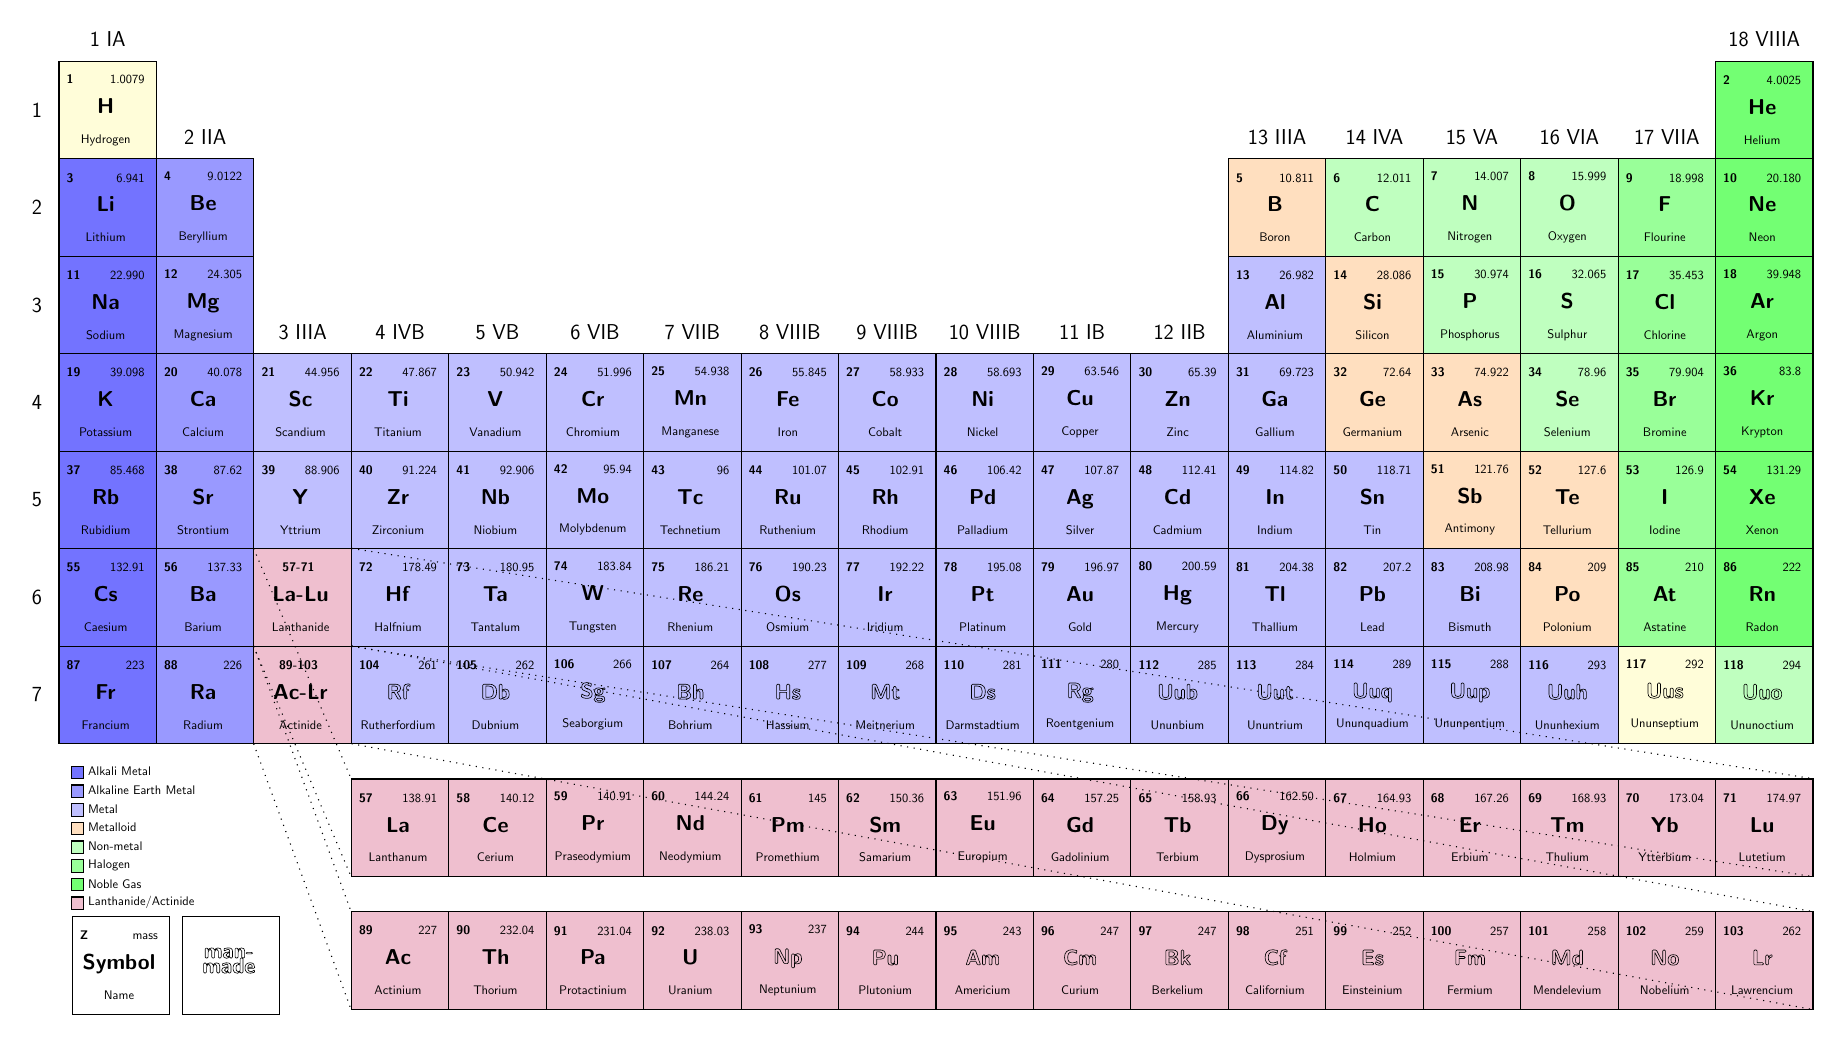
\begin{tikzpicture}[font=\sffamily, scale=0.45, transform shape]

%% Fill Color Styles
  \tikzstyle{ElementFill} = [fill=yellow!15]
  \tikzstyle{AlkaliMetalFill} = [fill=blue!55]
  \tikzstyle{AlkalineEarthMetalFill} = [fill=blue!40]
  \tikzstyle{MetalFill} = [fill=blue!25]
  \tikzstyle{MetalloidFill} = [fill=orange!25]
  \tikzstyle{NonmetalFill} = [fill=green!25]
  \tikzstyle{HalogenFill} = [fill=green!40]
  \tikzstyle{NobleGasFill} = [fill=green!55]
  \tikzstyle{LanthanideActinideFill} = [fill=purple!25]

%% Element Styles
  \tikzstyle{Element} = [draw=black, ElementFill,
    minimum width=2.75cm, minimum height=2.75cm, node distance=2.75cm]
  \tikzstyle{AlkaliMetal} = [Element, AlkaliMetalFill]
  \tikzstyle{AlkalineEarthMetal} = [Element, AlkalineEarthMetalFill]
  \tikzstyle{Metal} = [Element, MetalFill]
  \tikzstyle{Metalloid} = [Element, MetalloidFill]
  \tikzstyle{Nonmetal} = [Element, NonmetalFill]
  \tikzstyle{Halogen} = [Element, HalogenFill]
  \tikzstyle{NobleGas} = [Element, NobleGasFill]
  \tikzstyle{LanthanideActinide} = [Element, LanthanideActinideFill]
  \tikzstyle{PeriodLabel} = [font={\sffamily\LARGE}, node distance=2.0cm]
  \tikzstyle{GroupLabel} = [font={\sffamily\LARGE}, minimum width=2.75cm, node distance=2.0cm]
  \tikzstyle{TitleLabel} = [font={\sffamily\Huge\bfseries}]

%% Group 1 - IA
  \node[name=H, Element] {\NaturalElementTextFormat{1}{1.0079}{H}{Hydrogen}};
  \node[name=Li, below of=H, AlkaliMetal] {\NaturalElementTextFormat{3}{6.941}{Li}{Lithium}};
  \node[name=Na, below of=Li, AlkaliMetal] {\NaturalElementTextFormat{11}{22.990}{Na}{Sodium}};
  \node[name=K, below of=Na, AlkaliMetal] {\NaturalElementTextFormat{19}{39.098}{K}{Potassium}};
  \node[name=Rb, below of=K, AlkaliMetal] {\NaturalElementTextFormat{37}{85.468}{Rb}{Rubidium}};
  \node[name=Cs, below of=Rb, AlkaliMetal] {\NaturalElementTextFormat{55}{132.91}{Cs}{Caesium}};
  \node[name=Fr, below of=Cs, AlkaliMetal] {\NaturalElementTextFormat{87}{223}{Fr}{Francium}};

%% Group 2 - IIA
  \node[name=Be, right of=Li, AlkalineEarthMetal] {\NaturalElementTextFormat{4}{9.0122}{Be}{Beryllium}};
  \node[name=Mg, below of=Be, AlkalineEarthMetal] {\NaturalElementTextFormat{12}{24.305}{Mg}{Magnesium}};
  \node[name=Ca, below of=Mg, AlkalineEarthMetal] {\NaturalElementTextFormat{20}{40.078}{Ca}{Calcium}};
  \node[name=Sr, below of=Ca, AlkalineEarthMetal] {\NaturalElementTextFormat{38}{87.62}{Sr}{Strontium}};
  \node[name=Ba, below of=Sr, AlkalineEarthMetal] {\NaturalElementTextFormat{56}{137.33}{Ba}{Barium}};
  \node[name=Ra, below of=Ba, AlkalineEarthMetal] {\NaturalElementTextFormat{88}{226}{Ra}{Radium}};

%% Group 3 - IIIB
  \node[name=Sc, right of=Ca, Metal] {\NaturalElementTextFormat{21}{44.956}{Sc}{Scandium}};
  \node[name=Y, below of=Sc, Metal] {\NaturalElementTextFormat{39}{88.906}{Y}{Yttrium}};
  \node[name=LaLu, below of=Y, LanthanideActinide] {\NaturalElementTextFormat{57-71}{}{La-Lu}{Lanthanide}};
  \node[name=AcLr, below of=LaLu, LanthanideActinide] {\NaturalElementTextFormat{89-103}{}{Ac-Lr}{Actinide}};

%% Group 4 - IVB
  \node[name=Ti, right of=Sc, Metal] {\NaturalElementTextFormat{22}{47.867}{Ti}{Titanium}};
  \node[name=Zr, below of=Ti, Metal] {\NaturalElementTextFormat{40}{91.224}{Zr}{Zirconium}};
  \node[name=Hf, below of=Zr, Metal] {\NaturalElementTextFormat{72}{178.49}{Hf}{Halfnium}};
  \node[name=Rf, below of=Hf, Metal] {\SyntheticElementTextFormat{104}{261}{Rf}{Rutherfordium}};

%% Group 5 - VB
  \node[name=V, right of=Ti, Metal] {\NaturalElementTextFormat{23}{50.942}{V}{Vanadium}};
  \node[name=Nb, below of=V, Metal] {\NaturalElementTextFormat{41}{92.906}{Nb}{Niobium}};
  \node[name=Ta, below of=Nb, Metal] {\NaturalElementTextFormat{73}{180.95}{Ta}{Tantalum}};
  \node[name=Db, below of=Ta, Metal] {\SyntheticElementTextFormat{105}{262}{Db}{Dubnium}};

%% Group 6 - VIB
  \node[name=Cr, right of=V, Metal] {\NaturalElementTextFormat{24}{51.996}{Cr}{Chromium}};
  \node[name=Mo, below of=Cr, Metal] {\NaturalElementTextFormat{42}{95.94}{Mo}{Molybdenum}};
  \node[name=W, below of=Mo, Metal] {\NaturalElementTextFormat{74}{183.84}{W}{Tungsten}};
  \node[name=Sg, below of=W, Metal] {\SyntheticElementTextFormat{106}{266}{Sg}{Seaborgium}};

%% Group 7 - VIIB
  \node[name=Mn, right of=Cr, Metal] {\NaturalElementTextFormat{25}{54.938}{Mn}{Manganese}};
  \node[name=Tc, below of=Mn, Metal] {\NaturalElementTextFormat{43}{96}{Tc}{Technetium}};
  \node[name=Re, below of=Tc, Metal] {\NaturalElementTextFormat{75}{186.21}{Re}{Rhenium}};
  \node[name=Bh, below of=Re, Metal] {\SyntheticElementTextFormat{107}{264}{Bh}{Bohrium}};

%% Group 8 - VIIIB
  \node[name=Fe, right of=Mn, Metal] {\NaturalElementTextFormat{26}{55.845}{Fe}{Iron}};
  \node[name=Ru, below of=Fe, Metal] {\NaturalElementTextFormat{44}{101.07}{Ru}{Ruthenium}};
  \node[name=Os, below of=Ru, Metal] {\NaturalElementTextFormat{76}{190.23}{Os}{Osmium}};
  \node[name=Hs, below of=Os, Metal] {\SyntheticElementTextFormat{108}{277}{Hs}{Hassium}};

%% Group 9 - VIIIB
  \node[name=Co, right of=Fe, Metal] {\NaturalElementTextFormat{27}{58.933}{Co}{Cobalt}};
  \node[name=Rh, below of=Co, Metal] {\NaturalElementTextFormat{45}{102.91}{Rh}{Rhodium}};
  \node[name=Ir, below of=Rh, Metal] {\NaturalElementTextFormat{77}{192.22}{Ir}{Iridium}};
  \node[name=Mt, below of=Ir, Metal] {\SyntheticElementTextFormat{109}{268}{Mt}{Meitnerium}};

%% Group 10 - VIIIB
  \node[name=Ni, right of=Co, Metal] {\NaturalElementTextFormat{28}{58.693}{Ni}{Nickel}};
  \node[name=Pd, below of=Ni, Metal] {\NaturalElementTextFormat{46}{106.42}{Pd}{Palladium}};
  \node[name=Pt, below of=Pd, Metal] {\NaturalElementTextFormat{78}{195.08}{Pt}{Platinum}};
  \node[name=Ds, below of=Pt, Metal] {\SyntheticElementTextFormat{110}{281}{Ds}{Darmstadtium}};

%% Group 11 - IB
  \node[name=Cu, right of=Ni, Metal] {\NaturalElementTextFormat{29}{63.546}{Cu}{Copper}};
  \node[name=Ag, below of=Cu, Metal] {\NaturalElementTextFormat{47}{107.87}{Ag}{Silver}};
  \node[name=Au, below of=Ag, Metal] {\NaturalElementTextFormat{79}{196.97}{Au}{Gold}};
  \node[name=Rg, below of=Au, Metal] {\SyntheticElementTextFormat{111}{280}{Rg}{Roentgenium}};

%% Group 12 - IIB
  \node[name=Zn, right of=Cu, Metal] {\NaturalElementTextFormat{30}{65.39}{Zn}{Zinc}};
  \node[name=Cd, below of=Zn, Metal] {\NaturalElementTextFormat{48}{112.41}{Cd}{Cadmium}};
  \node[name=Hg, below of=Cd, Metal] {\NaturalElementTextFormat{80}{200.59}{Hg}{Mercury}};
  \node[name=Uub, below of=Hg, Metal] {\SyntheticElementTextFormat{112}{285}{Uub}{Ununbium}};

%% Group 13 - IIIA
  \node[name=Ga, right of=Zn, Metal] {\NaturalElementTextFormat{31}{69.723}{Ga}{Gallium}};
  \node[name=Al, above of=Ga, Metal] {\NaturalElementTextFormat{13}{26.982}{Al}{Aluminium}};
  \node[name=B, above of=Al, Metalloid] {\NaturalElementTextFormat{5}{10.811}{B}{Boron}};
  \node[name=In, below of=Ga, Metal] {\NaturalElementTextFormat{49}{114.82}{In}{Indium}};
  \node[name=Tl, below of=In, Metal] {\NaturalElementTextFormat{81}{204.38}{Tl}{Thallium}};
  \node[name=Uut, below of=Tl, Metal] {\SyntheticElementTextFormat{113}{284}{Uut}{Ununtrium}};

%% Group 14 - IVA
  \node[name=C, right of=B, Nonmetal] {\NaturalElementTextFormat{6}{12.011}{C}{Carbon}};
  \node[name=Si, below of=C, Metalloid] {\NaturalElementTextFormat{14}{28.086}{Si}{Silicon}};
  \node[name=Ge, below of=Si, Metalloid] {\NaturalElementTextFormat{32}{72.64}{Ge}{Germanium}};
  \node[name=Sn, below of=Ge, Metal] {\NaturalElementTextFormat{50}{118.71}{Sn}{Tin}};
  \node[name=Pb, below of=Sn, Metal] {\NaturalElementTextFormat{82}{207.2}{Pb}{Lead}};
  \node[name=Uuq, below of=Pb, Metal] {\SyntheticElementTextFormat{114}{289}{Uuq}{Ununquadium}};

%% Group 15 - VA
  \node[name=N, right of=C, Nonmetal] {\NaturalElementTextFormat{7}{14.007}{N}{Nitrogen}};
  \node[name=P, below of=N, Nonmetal] {\NaturalElementTextFormat{15}{30.974}{P}{Phosphorus}};
  \node[name=As, below of=P, Metalloid] {\NaturalElementTextFormat{33}{74.922}{As}{Arsenic}};
  \node[name=Sb, below of=As, Metalloid] {\NaturalElementTextFormat{51}{121.76}{Sb}{Antimony}};
  \node[name=Bi, below of=Sb, Metal] {\NaturalElementTextFormat{83}{208.98}{Bi}{Bismuth}};
  \node[name=Uup, below of=Bi, Metal] {\SyntheticElementTextFormat{115}{288}{Uup}{Ununpentium}};

%% Group 16 - VIA
  \node[name=O, right of=N, Nonmetal] {\NaturalElementTextFormat{8}{15.999}{O}{Oxygen}};
  \node[name=S, below of=O, Nonmetal] {\NaturalElementTextFormat{16}{32.065}{S}{Sulphur}};
  \node[name=Se, below of=S, Nonmetal] {\NaturalElementTextFormat{34}{78.96}{Se}{Selenium}};
  \node[name=Te, below of=Se, Metalloid] {\NaturalElementTextFormat{52}{127.6}{Te}{Tellurium}};
  \node[name=Po, below of=Te, Metalloid] {\NaturalElementTextFormat{84}{209}{Po}{Polonium}};
  \node[name=Uuh, below of=Po, Metal] {\SyntheticElementTextFormat{116}{293}{Uuh}{Ununhexium}};

%% Group 17 - VIIA
  \node[name=F, right of=O, Halogen] {\NaturalElementTextFormat{9}{18.998}{F}{Flourine}};
  \node[name=Cl, below of=F, Halogen] {\NaturalElementTextFormat{17}{35.453}{Cl}{Chlorine}};
  \node[name=Br, below of=Cl, Halogen] {\NaturalElementTextFormat{35}{79.904}{Br}{Bromine}};
  \node[name=I, below of=Br, Halogen] {\NaturalElementTextFormat{53}{126.9}{I}{Iodine}};
  \node[name=At, below of=I, Halogen] {\NaturalElementTextFormat{85}{210}{At}{Astatine}};
  \node[name=Uus, below of=At, Element] {\SyntheticElementTextFormat{117}{292}{Uus}{Ununseptium}}; 

%% Group 18 - VIIIA
  \node[name=Ne, right of=F, NobleGas] {\NaturalElementTextFormat{10}{20.180}{Ne}{Neon}};
  \node[name=He, above of=Ne, NobleGas] {\NaturalElementTextFormat{2}{4.0025}{He}{Helium}};
  \node[name=Ar, below of=Ne, NobleGas] {\NaturalElementTextFormat{18}{39.948}{Ar}{Argon}};
  \node[name=Kr, below of=Ar, NobleGas] {\NaturalElementTextFormat{36}{83.8}{Kr}{Krypton}};
  \node[name=Xe, below of=Kr, NobleGas] {\NaturalElementTextFormat{54}{131.29}{Xe}{Xenon}};
  \node[name=Rn, below of=Xe, NobleGas] {\NaturalElementTextFormat{86}{222}{Rn}{Radon}};
  \node[name=Uuo, below of=Rn, Nonmetal] {\SyntheticElementTextFormat{118}{294}{Uuo}{Ununoctium}}; 

%% Period
  \node[name=Period1, left of=H, PeriodLabel] {1};
  \node[name=Period2, left of=Li, PeriodLabel] {2};
  \node[name=Period3, left of=Na, PeriodLabel] {3}; 
  \node[name=Period4, left of=K, PeriodLabel] {4}; 
  \node[name=Period5, left of=Rb, PeriodLabel] {5};
  \node[name=Period6, left of=Cs, PeriodLabel] {6};
  \node[name=Period7, left of=Fr, PeriodLabel] {7};

%% Group
  \node[name=Group1, above of=H, GroupLabel] {1 \hfill IA};
  \node[name=Group2, above of=Be, GroupLabel] {2 \hfill IIA};
  \node[name=Group3, above of=Sc, GroupLabel] {3 \hfill IIIA};
  \node[name=Group4, above of=Ti, GroupLabel] {4 \hfill IVB};
  \node[name=Group5, above of=V, GroupLabel] {5 \hfill VB};
  \node[name=Group6, above of=Cr, GroupLabel] {6 \hfill VIB};
  \node[name=Group7, above of=Mn, GroupLabel] {7 \hfill VIIB};
  \node[name=Group8, above of=Fe, GroupLabel] {8 \hfill VIIIB};
  \node[name=Group9, above of=Co, GroupLabel] {9 \hfill VIIIB};
  \node[name=Group10, above of=Ni, GroupLabel] {10 \hfill VIIIB};
  \node[name=Group11, above of=Cu, GroupLabel] {11 \hfill IB};
  \node[name=Group12, above of=Zn, GroupLabel] {12 \hfill IIB};
  \node[name=Group13, above of=B, GroupLabel] {13 \hfill IIIA};
  \node[name=Group14, above of=C, GroupLabel] {14 \hfill IVA};
  \node[name=Group15, above of=N, GroupLabel] {15 \hfill VA};
  \node[name=Group16, above of=O, GroupLabel] {16 \hfill VIA};
  \node[name=Group17, above of=F, GroupLabel] {17 \hfill VIIA};
  \node[name=Group18, above of=He, GroupLabel] {18 \hfill VIIIA};

%% Lanthanide
  \node[name=La, below of=Rf, LanthanideActinide, yshift=-1cm] {\NaturalElementTextFormat{57}{138.91}{La}{Lanthanum}};
  \node[name=Ce, right of=La, LanthanideActinide] {\NaturalElementTextFormat{58}{140.12}{Ce}{Cerium}};
  \node[name=Pr, right of=Ce, LanthanideActinide] {\NaturalElementTextFormat{59}{140.91}{Pr}{Praseodymium}};
  \node[name=Nd, right of=Pr, LanthanideActinide] {\NaturalElementTextFormat{60}{144.24}{Nd}{Neodymium}};
  \node[name=Pm, right of=Nd, LanthanideActinide] {\NaturalElementTextFormat{61}{145}{Pm}{Promethium}};
  \node[name=Sm, right of=Pm, LanthanideActinide] {\NaturalElementTextFormat{62}{150.36}{Sm}{Samarium}};
  \node[name=Eu, right of=Sm, LanthanideActinide] {\NaturalElementTextFormat{63}{151.96}{Eu}{Europium}};
  \node[name=Gd, right of=Eu, LanthanideActinide] {\NaturalElementTextFormat{64}{157.25}{Gd}{Gadolinium}};
  \node[name=Tb, right of=Gd, LanthanideActinide] {\NaturalElementTextFormat{65}{158.93}{Tb}{Terbium}};
  \node[name=Dy, right of=Tb, LanthanideActinide] {\NaturalElementTextFormat{66}{162.50}{Dy}{Dysprosium}};
  \node[name=Ho, right of=Dy, LanthanideActinide] {\NaturalElementTextFormat{67}{164.93}{Ho}{Holmium}};
  \node[name=Er, right of=Ho, LanthanideActinide] {\NaturalElementTextFormat{68}{167.26}{Er}{Erbium}};
  \node[name=Tm, right of=Er, LanthanideActinide] {\NaturalElementTextFormat{69}{168.93}{Tm}{Thulium}};
  \node[name=Yb, right of=Tm, LanthanideActinide] {\NaturalElementTextFormat{70}{173.04}{Yb}{Ytterbium}};
  \node[name=Lu, right of=Yb, LanthanideActinide] {\NaturalElementTextFormat{71}{174.97}{Lu}{Lutetium}};

%% Actinide
  \node[name=Ac, below of=La, LanthanideActinide, yshift=-1cm] {\NaturalElementTextFormat{89}{227}{Ac}{Actinium}};
  \node[name=Th, right of=Ac, LanthanideActinide] {\NaturalElementTextFormat{90}{232.04}{Th}{Thorium}};
  \node[name=Pa, right of=Th, LanthanideActinide] {\NaturalElementTextFormat{91}{231.04}{Pa}{Protactinium}};
  \node[name=U, right of=Pa, LanthanideActinide] {\NaturalElementTextFormat{92}{238.03}{U}{Uranium}};
  \node[name=Np, right of=U, LanthanideActinide] {\SyntheticElementTextFormat{93}{237}{Np}{Neptunium}};
  \node[name=Pu, right of=Np, LanthanideActinide] {\SyntheticElementTextFormat{94}{244}{Pu}{Plutonium}};
  \node[name=Am, right of=Pu, LanthanideActinide] {\SyntheticElementTextFormat{95}{243}{Am}{Americium}};
  \node[name=Cm, right of=Am, LanthanideActinide] {\SyntheticElementTextFormat{96}{247}{Cm}{Curium}};
  \node[name=Bk, right of=Cm, LanthanideActinide] {\SyntheticElementTextFormat{97}{247}{Bk}{Berkelium}};
  \node[name=Cf, right of=Bk, LanthanideActinide] {\SyntheticElementTextFormat{98}{251}{Cf}{Californium}};
  \node[name=Es, right of=Cf, LanthanideActinide] {\SyntheticElementTextFormat{99}{252}{Es}{Einsteinium}};
  \node[name=Fm, right of=Es, LanthanideActinide] {\SyntheticElementTextFormat{100}{257}{Fm}{Fermium}};
  \node[name=Md, right of=Fm, LanthanideActinide] {\SyntheticElementTextFormat{101}{258}{Md}{Mendelevium}};
  \node[name=No, right of=Md, LanthanideActinide] {\SyntheticElementTextFormat{102}{259}{No}{Nobelium}};
  \node[name=Lr, right of=No, LanthanideActinide] {\SyntheticElementTextFormat{103}{262}{Lr}{Lawrencium}};

%% Draw dotted lines connecting Lanthanide breakout to main table
  \draw (LaLu.north west) edge[dotted] (La.north west)
        (LaLu.north east) edge[dotted] (Lu.north east)
        (LaLu.south west) edge[dotted] (La.south west)
        (LaLu.south east) edge[dotted] (Lu.south east);
%% Draw dotted lines connecting Actinide breakout to main table
  \draw (AcLr.north west) edge[dotted] (Ac.north west)
        (AcLr.north east) edge[dotted] (Lr.north east)
        (AcLr.south west) edge[dotted] (Ac.south west)
        (AcLr.south east) edge[dotted] (Lr.south east);

%% Legend
  \draw[black, AlkaliMetalFill] ($(La.north -| Fr.west) + (1em,-0.0em)$)
    rectangle +(1em, 1em) node[right, yshift=-1ex]{Alkali Metal};
  \draw[black, AlkalineEarthMetalFill] ($(La.north -| Fr.west) + (1em,-1.5em)$)
    rectangle +(1em, 1em) node[right, yshift=-1ex]{Alkaline Earth Metal};
  \draw[black, MetalFill] ($(La.north -| Fr.west) + (1em,-3.0em)$)
    rectangle +(1em, 1em) node[right, yshift=-1ex]{Metal};
  \draw[black, MetalloidFill] ($(La.north -| Fr.west) + (1em,-4.5em)$)
    rectangle +(1em, 1em) node[right, yshift=-1ex]{Metalloid};
  \draw[black, NonmetalFill] ($(La.north -| Fr.west) + (1em,-6.0em)$)
    rectangle +(1em, 1em) node[right, yshift=-1ex]{Non-metal};
  \draw[black, HalogenFill] ($(La.north -| Fr.west) + (1em,-7.5em)$)
    rectangle +(1em, 1em) node[right, yshift=-1ex]{Halogen};
  \draw[black, NobleGasFill] ($(La.north -| Fr.west) + (1em,-9.0em)$)
    rectangle +(1em, 1em) node[right, yshift=-1ex]{Noble Gas};
  \draw[black, LanthanideActinideFill] ($(La.north -| Fr.west) + (1em,-10.5em)$)
    rectangle +(1em, 1em) node[right, yshift=-1ex]{Lanthanide/Actinide};

  \node at ($(La.north -| Fr.west) + (5em,-15em)$) [name=elementLegend, Element, fill=white]
    {\NaturalElementTextFormat{Z}{mass}{Symbol}{Name}};
  \node[Element, fill=white, right of=elementLegend, xshift=1em]
    {\SyntheticElementTextFormat{}{}{man-made}{}} ;
\end{tikzpicture}
}
{\footnotesize D. Mendeleev, I. Griffin}
\end{frame}

\begin{frame}
  \frametitle{What sets the relative abundances of elements?}
  \begin{itemize}
  \item Observations of the sun one major way to measure abundances.
  \end{itemize}
  \begin{center}
    \resizebox{12cm}{!}{
      \begin{tikzpicture}
        \node[inner sep=0pt] (sun) at (0,0)
        {\includegraphics[width=0.25\columnwidth]{sun-cropped}};
        \draw[ultra thick, blue] (0, -1) -- ++(-6,-1);
        \draw[ultra thick, blue] (0, -1) -- ++(6, -1);
        \node[draw, blue, inner sep=0pt] (abun) at (0, -3)
        {\includegraphics[width=\columnwidth]{1920px-Elements_abundance_bars}};
        \node at (3, -3) {This is on a log scale!};
        \node at (5, -4.5) {\small atomic mass};
        \node[rotate=90] at (-6.5, -3) {\small rel. abun.};
      \end{tikzpicture}
    }
  \end{center}
  Image credit: NASA/APOD, Wikipedia
\end{frame}

\begin{frame}
  \frametitle{The Many Sources of the Elements in Our Universe}
  \begin{center}
    \resizebox{12cm}{!}{
      \begin{tikzpicture}
        \node[inner sep=0pt] at (0,0)
        {\includegraphics[width=\columnwidth]{Nucleosynthesis_periodic_table}};
        \draw[blue,visible on=<2->] (-2,1.5) circle (0.75);
        \draw[blue,visible on=<2->] (-0.25,2.5) circle (0.75);
      \end{tikzpicture}
      }
    \end{center}
    Image credit: Jennifer Johnson. Adapted by Wikipedia user cmglee.
\end{frame}

\begin{frame}
 \frametitle{The r-process}
 \begin{center}
  \includegraphics[width=0.9\textwidth]{skynet_ye_0p13/frame_0001}
 \end{center}
 Courtesy of J. Lippuner
\end{frame}

\begin{frame}
 \frametitle{The r-process}
 \begin{center}
   % \includegraphics[width=0.9\textwidth]{skynet_ye_0p13/frame_0001}
   \animategraphics[width=0.9\textwidth,every=5,autoplay,loop,controls]
   {5}{skynet_ye_0p13/frame_}{0001}{0108}
 \end{center}
 Courtesy of J. Lippuner
\end{frame}

\begin{frame}
 \frametitle{The r-process}
 \begin{center}
   \includegraphics[width=0.9\textwidth]{skynet_ye_0p13/frame_0108}
 \end{center}
 Courtesy of J. Lippuner
\end{frame}

\begin{frame}
  \frametitle{Nucleosynthesis in SN1987A}
  \begin{columns}
    \begin{column}{4cm}
      \begin{center}
        \includegraphics[width=\columnwidth]{SN1987A_hubble_cropped}\\
        NASA/HUBBLE
      \end{center}
    \end{column}
    \begin{column}{8cm}
      \begin{center}
        \includegraphics[width=\columnwidth]{rank-sn1987a-IR-spectrum}\\
        Rank et al. \textit{Nature} \textbf{331}, 505–506 (1988)
      \end{center}
    \end{column}
  \end{columns}
\end{frame}

\begin{frame}
  \frametitle{The Rare-Earth Peak and Metal-Poor Stars}
  \begin{columns}
    \begin{column}{6cm}
      \begin{center}
        \includegraphics[width=\columnwidth]{cowan-metal-poor-stars}
      \end{center}
      J. J. Cowan
    \end{column}
    \begin{column}{6cm}
      \begin{itemize}
      \item Spectra from many stars available.
      \item Stars with not too many heavy elements show an interesting,
        repeatable pattern, which shows up in our sun too!
      \item At least one source (beyond CCSN) needed, possibly more
        than one!
      \end{itemize}      
    \end{column}
  \end{columns}
\end{frame}

\begin{frame}
  \frametitle{Striking Cosmic Gold With Neutron Star Mergers}
  \begin{center}
    \includegraphics[width=0.9\textwidth]{quantagold_19201}
  \end{center}
  Ashley Mackenzie for Quanta Magazine, March 23, 2017
\end{frame}

% \begin{frame}
%   \frametitle{Observations Galore!}
%   \begin{center}
%     \includegraphics[height=7cm]{abbot-timeline}
%   \end{center}
%   Abbot+, 2017
% \end{frame}

\begin{frame}
  \frametitle{Neutron Stars}
  \begin{center}
    \includegraphics[width=0.9\textwidth]{ns-manhattan}
  \end{center}
  Wikimedia Commons
\end{frame}

\begin{frame}
  \frametitle{Neutron Star Mergers: A 2+ Component Model}
  \begin{columns}
    \begin{column}{6cm}
      \begin{center}
        % \includegraphics[width=0.9\textwidth]{frames/betabin_000}
        \animategraphics[width=0.9\textwidth,every=10,autoplay,loop,controls]
        {5}{frames/betabin_}{000}{374}
      \end{center}
    \end{column}
    \begin{column}{6cm}
      \begin{center}
        \resizebox{\columnwidth}{!}{
          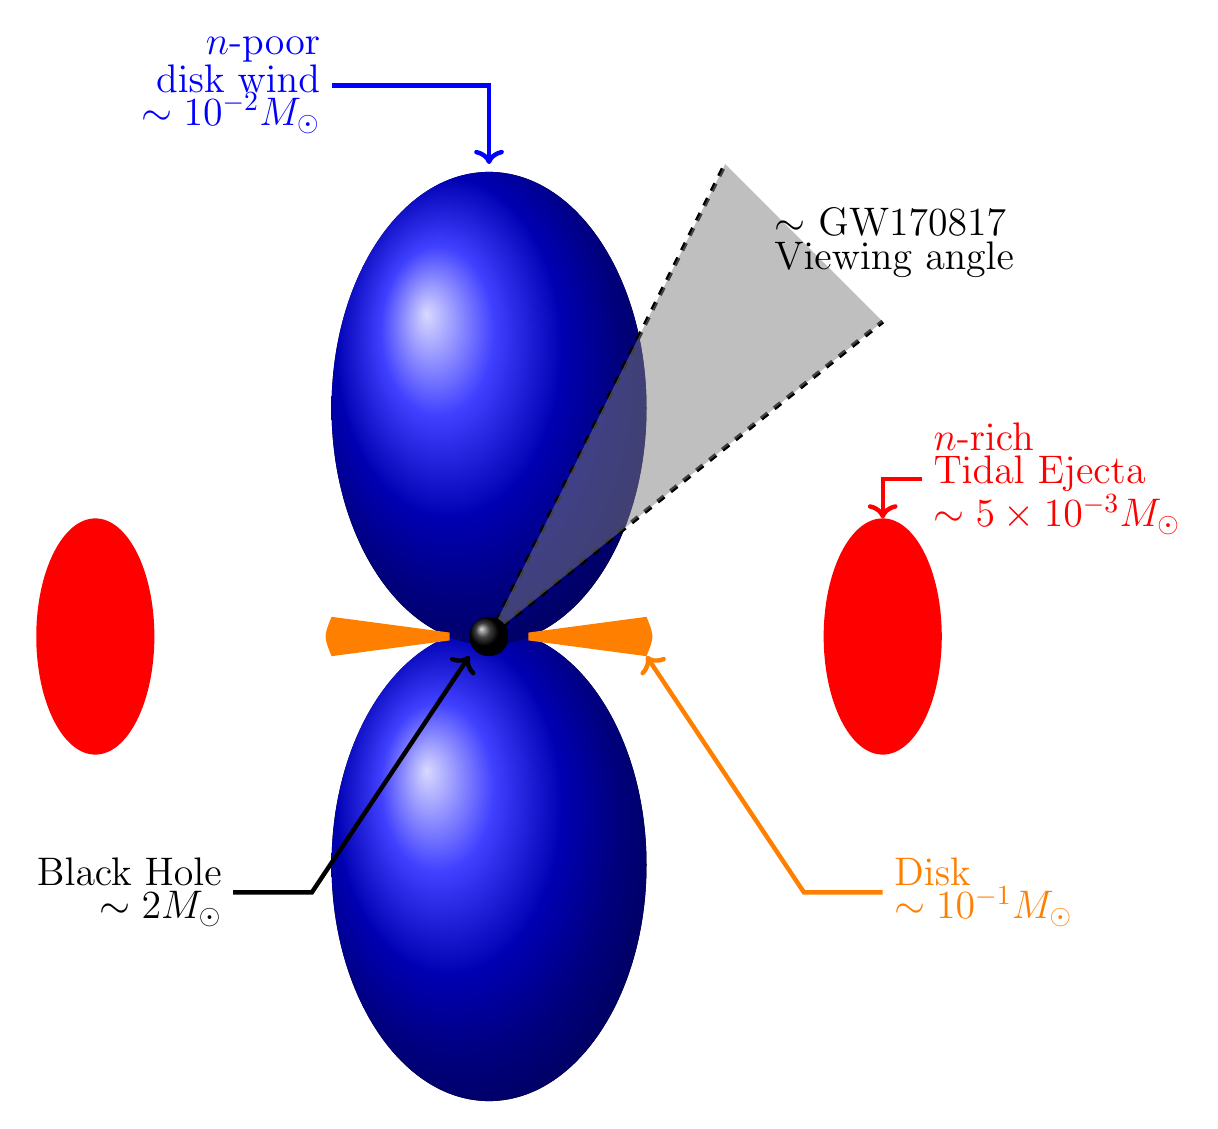
\begin{tikzpicture}
            \coordinate (origin) at (0,0);
            \pgfmathsetmacro{\dbx}{0.5}
            \pgfmathsetmacro{\dby}{0.05}
            \pgfmathsetmacro{\dex}{2.}
            \pgfmathsetmacro{\dey}{0.25}
            \pgfmathsetmacro{\dcc}{2.1}
            \pgfmathsetmacro{\tcx}{5.0}

            \foreach \i in {-1,1}
            {
              \fill[ball color=blue] (0, \i*2.9) ellipse (2 and 3);
            }

            \foreach \i in {-1,1}
            {
              % disk
              \fill[color=orange]
              (\i*\dbx,\dby) -- (\i*\dex,\dey)
              .. controls (\i*\dcc,0) .. (\i*\dex,-\dey)
              -- (\i*\dbx,-\dby) -- cycle;

              % tidal ejecta
              \fill[color=red] (\i*\tcx,0) ellipse (0.75 and 1.5);
            }

            % viewing
            \draw[dashed,ultra thick,black] (origin) -- (5,4);
            \draw[dashed,ultra thick,black] (origin) -- (3,6);
            \fill[color=gray,opacity=0.5] (origin) -- (5,4) -- (3,6) -- cycle;
            \node[right,align=left] at (3.5,5)
            {\Large $\sim$ GW170817\\ \Large Viewing angle};

            % bh
            \shade[ball color=black] (origin) circle (0.25);

            % text
            \draw[<-,red, ultra thick] (\tcx,1.5)
            -- ++(0.,0.5) -- ++(0.5,0)
            node[right,align=left]
            {\Large \color{red}$n$-rich\\\Large Tidal Ejecta\\ \Large $\sim 5\times 10^{-3}M_{\odot}$};

            \draw[<-,blue, ultra thick] (0,6) -- ++(0,1) -- ++(-2,0)
            node[left,align=right]
            {\Large \color{blue}$n$-poor\\\Large disk wind\\\Large $\sim 10^{-2}M_{\odot}$};

            \draw[<-,orange, ultra thick] (\dex,-\dey)
            -- ++(2,-3) -- ++(1,0)
            node[right,align=left]
            {\Large \color{orange}Disk\\\Large $\sim 10^{-1}M_{\odot}$};

            \draw[<-,black, ultra thick] (-0.25,-0.25)
            -- ++(-2,-3) -- ++(-1,0)
            node[left,align=right]
            {\Large \color{black}Black Hole\\ \Large $\sim 2 M_{\odot}$};
          \end{tikzpicture}
        }
      \end{center}
    \end{column}
  \end{columns}
  \begin{tiny}
    Co-design summer school, 2016
  \end{tiny}
\end{frame}

\begin{frame}
  \frametitle{Opacity}
  %\setlength{\unitlength}{1cm}
  \resizebox{12cm}{!}{
    \begin{tikzpicture}
      \node[inner sep=0pt] (rp) at (0,0)
      {\includegraphics[width=10cm]{skynet_ye_0p13/frame_0108}};
      \draw[ultra thick,red,<-] (1.5,-2) -- (2,-2.85)
      -- (2.25, -2.85) node[right] {\tiny Opaque to visible light};
      \draw[ultra thick,red,<-] (0.85,-2) -- (0.5,-2.85)
      -- (0.25,-2.85) node[left] {\tiny Not opaque};
    \end{tikzpicture}
  }
\end{frame}

\begin{frame}
  \frametitle{The Kilonova}
  \begin{center}
    \includegraphics[width=10cm]{swope-image}
  \end{center}
  M2H/UC Santa Cruz and Carnegie Observatories/Ryan Foley
\end{frame}

\begin{frame}
  \frametitle{Are NS Mergers the Only Source?}
  \begin{columns}
    \begin{column}{6cm}
      \begin{itemize}
      \item NSs take time to form, then for their orbit to in-spiral.
      % \item Abundance of Fe relative to Hydrogen is rough measure of
      %   age of a star.
      % \item Abundance of Eu relative to Fe is rough measure of
      %   enrichment.
      \item Our understanding of this delay-time does not match rough
        enrichment vs time observed in galactic halo and disk stars.
      \item Perhaps another enrichment source that can happen at
        earlier times is needed?
      \item Alternatively, our understanding of binary evolution could
        be (probably is) wrong!
      \end{itemize}
    \end{column}
    \begin{column}{6cm}
      \begin{center}
        \includegraphics[width=0.9\columnwidth]{cotedelaytime}
      \end{center}
      Cote et al., ApJ \textbf{875} 106 (2019)
    \end{column}
  \end{columns}
\end{frame}

\begin{frame}
  \frametitle{Accretion disks in supernovae?}
  \begin{columns}
    \begin{column}{6cm}
      \begin{center}
        \includegraphics[width=\columnwidth]{beppo-sax-light-curve}
      \end{center}
      Ruffini et al. BepoSAX telescope. arXiv:0705.2456
    \end{column}
    \begin{column}{6cm}
      \begin{center}
        \includegraphics[width=\columnwidth]{2250px-SN_1998bw}\\
        European Southern Observatory
      \end{center}
    \end{column}
  \end{columns}
\end{frame}

\begin{frame}
  \frametitle{Collapsars: Failed Supernovae}
  \begin{columns}
    \begin{column}{5cm}
      \begin{itemize}
      \item Accretion times $t\sim 10s$
      \item $\dot{M}$ between
        \begin{itemize}
        \item $10^{-4} M_\odot/s$
        \item $10^{-1} M_\odot/s$ 
        \end{itemize}
      \item $\rho \sim 10^{10}$ g$/$cm$^3$
      \end{itemize}
      \resizebox{\columnwidth}{!}{
        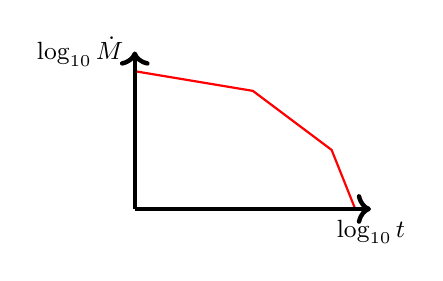
\begin{tikzpicture}
          \draw[thick,red]
          (0,1.75) -- (1.5,1.5) -- (2.5,0.75) -- (2.8,0);

          \coordinate (origin) at (0,0);
          \draw[ultra thick,->]
          (origin) -- ++(3,0)
          node[below] {\small $\log_{10}t$};
          \draw[ultra thick,->]
          (origin) -- ++(0,2)
          node[left] {\small $\log_{10}\dot{M}$};
        \end{tikzpicture}
      }
      \begin{tiny}
        Siegel, Barnes, Metzger. Nature \textbf{241} (2019)
      \end{tiny}
    \end{column}
    \begin{column}{7cm}
      \resizebox{\columnwidth}{!}{
        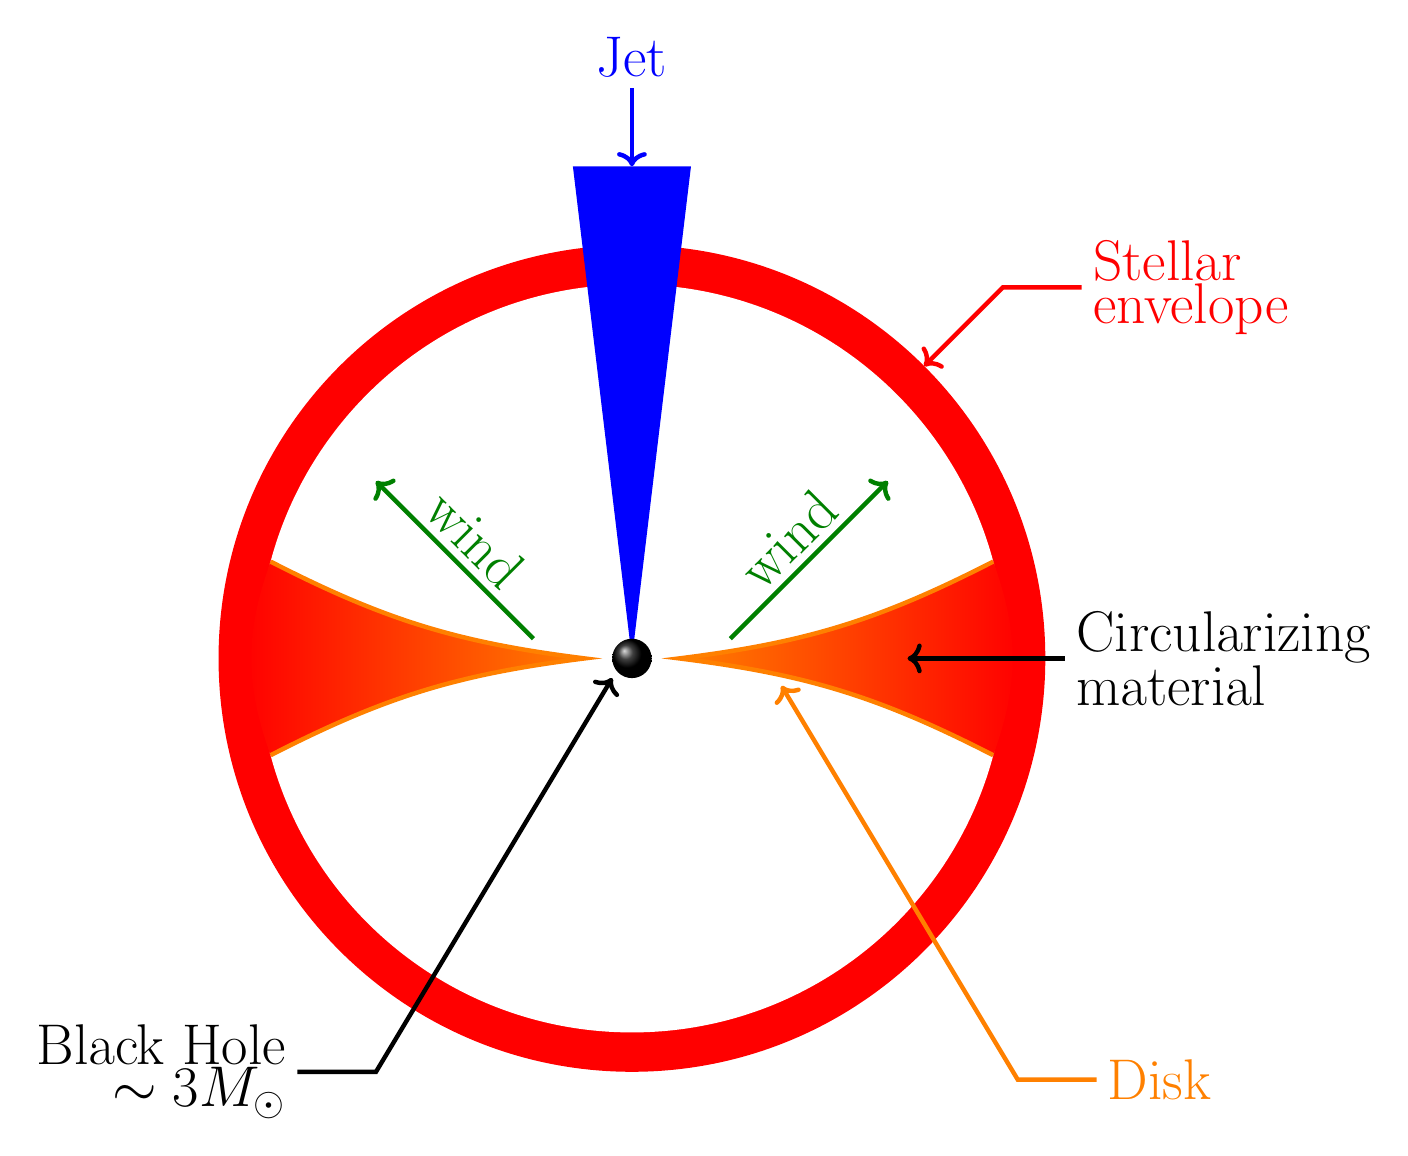
\begin{tikzpicture}
          \coordinate (origin) at (0,0);
          \pgfmathsetmacro{\pi}{3.14159}
          \pgfmathsetmacro{\dbx}{0.5}
          \pgfmathsetmacro{\dby}{0.05}
          \pgfmathsetmacro{\dex}{2.}
          \pgfmathsetmacro{\dey}{0.25}
          \pgfmathsetmacro{\dcc}{2.1}
          \pgfmathsetmacro{\tcx}{5.0}
          \pgfmathsetmacro{\rstar}{5}
          \pgfmathsetmacro{\wstar}{0.25}
          \pgfmathsetmacro{\wjet}{0.75}
          \pgfmathsetmacro{\tangle}{{45}}
          \pgfmathsetmacro{\tsx}{{(\rstar+\wstar)*cos(\tangle)}}
          \pgfmathsetmacro{\tsy}{{(\rstar+\wstar)*sin(\tangle)}}

          \pgfmathsetmacro{\cangle}{15}
          \pgfmathsetmacro{\cx}{(\rstar-\wstar)*cos(\cangle)}
          \pgfmathsetmacro{\cy}{(\rstar-\wstar)*sin(\cangle)}
          % \pgfmathsetmacro{\cend}{\dex + 0.1}
          \pgfmathsetmacro{\cend}{\dbx + 0.1}

          \newcommand{\msize}{\huge}

          % star
          \fill [color=red] (origin) circle (\rstar+\wstar);
          \fill [color=white] (origin) circle (\rstar-\wstar);

          % circularization
          \fill[color=red,
          left color=orange,
          middle color=orange,
          right color=red]
          (\cx,\cy) to [bend left=10] (\cend,0)
          to [bend left=10] (\cx,-\cy)
          to [bend right=20] cycle;
          
          \draw[orange,ultra thick]
          (\cx,\cy) to [bend left=10] (\cend, 0)
          to [bend left=10] (\cx,-\cy);

          \fill[color=red,
          right color=orange,
          middle color=orange,
          left color=red]
          (-\cx,\cy) to [bend right=10] (-\cend,0)
          to [bend right=10] (-\cx,-\cy)
          to [bend left=20] cycle;
          
          \draw[orange,ultra thick]
          (-\cx,\cy) to [bend right=10] (-\cend, 0)
          to [bend right=10] (-\cx,-\cy);

          % \foreach \i in {-1,1}
          % {
          %   % disk
          %   \fill[color=orange]
          %   (\i*\dbx,\dby) -- (\i*\dex,\dey)
          %   .. controls (\i*\dcc,0) .. (\i*\dex,-\dey)
          %   -- (\i*\dbx,-\dby) -- cycle;
          % }
          
          % jet
          \fill[color=blue] (origin) -- (-\wjet,1.25*\rstar) -- ++(2*\wjet,0) -- cycle;

          % bh
          \shade[ball color=black] (origin) circle (0.25);

          % wind
          \draw[deepgreen,ultra thick, ->]
          ({0.5*(\dbx + \dex)},\dey) -- ++(2,2);
          \draw ({0.5*(\dbx + \dex) + 1},{(\dey+1)})
          node[above,align=center,rotate=45]
          {\color{deepgreen}\msize wind};
          \draw[deepgreen,ultra thick, ->]
          ({-0.5*(\dbx + \dex)},\dey) -- ++(-2,2);
          \draw ({-(0.5*(\dbx + \dex) + 1)},{(\dey+1)})
          node[above,align=center,rotate=-45]
          {\color{deepgreen}\msize wind};          

          % text
          \draw[<-,orange, ultra thick] (\dex-0.1,-\dey-0.1)
          -- ++(3,-5) -- ++(1,0)
          node[right,align=left]
          {\msize \color{orange}Disk};
          
          \draw[<-,black, ultra thick] (-0.25,-0.25)
          -- ++(-3,-5) -- ++(-1,0)
          node[left,align=right]
          {\msize \color{black}Black Hole\\ \msize $\sim 3 M_{\odot}$};
          
          \draw[<-,red,ultra thick] (\tsx,\tsy)
          -- ++(1,1) -- ++(1,0)
          node[right,align=left]
          {\msize \color{red} Stellar\\ \msize envelope};

          \draw[<-,blue,ultra thick] (0, 1.25*\rstar) -- ++(0,1)
          node[above,align=center] {\msize \color{blue} Jet};

          \draw[<-,black,ultra thick]
          ({0.5*(\dex+\rstar)},0) -- ++(2,0) node[right,align=left]
          {\msize Circularizing\\ \msize material};
          
          \let\msize\undefined
        \end{tikzpicture}
      }
    \end{column}
  \end{columns}
\end{frame}

\begin{frame}
  \frametitle{This Work Focuses on the Disk}
  \begin{center}
    \resizebox{12.cm}{!}{
      \begin{tikzpicture}
        \filldraw[black] (0,0) rectangle ++(12,8);
        % \node[right,align=left] at (0,0.25){\color{red}\textbf{JMM}+, in prep.};
        \node[inner sep=0pt] (wind) at (3,4)
        {\includegraphics[width=0.5\textwidth]{wind-3d-render}};
        \node[inner sep=0pt,rectangle,blue,ultra thick] (disk) at (9,5)
        {\includegraphics[width=0.4\textwidth]{disk_image_no_text}};
        \draw[blue,ultra thick] (6.5,3.5) rectangle ++(5,3.);
        \draw[blue,ultra thick] (3,4) -- (6.5,6.5);
        \draw[blue,ultra thick] (3,4) -- (6.5,3.5);
      \end{tikzpicture}
      %\includegraphics[width=7cm]{disk_3d_render}
      }
  \end{center}
\end{frame}

\begin{frame}
  \frametitle{Neutrinos are required for nuclear reactions}
  \begin{center}
    \includegraphics[height=0.7\textheight]{Beta-minus_Decay}
  \end{center}
  Wikimedia Commons
\end{frame}

\begin{frame}
  \frametitle{Neutrino Transport Matters!}
  \begin{center}
    \includegraphics[height=0.8\textheight]{phoebus_movies/leptoneq/frame_0001}
  \end{center}
  \begin{tiny}
    \textbf{JMM}, B. R. Ryan, J. C. Dolence. ApJS \textbf{241} 30 (2019) \\
    New movie by Brandon Barker
  \end{tiny}
\end{frame}

\begin{frame}
  \frametitle{Neutrino Transport Matters!}
  \begin{center}
    % \includegraphics[height=0.8\textheight]{phoebus_movies/leptoneq/frame_0001}
    \animategraphics[height=0.8\textheight,every=5,autoplay,loop,controls]
    {5}{phoebus_movies/leptoneq/frame_}{0001}{0139}
  \end{center}
  \begin{tiny}
    \textbf{JMM}, B. R. Ryan, J. C. Dolence. ApJS \textbf{241} 30 (2019) \\
    New movie by Brandon Barker
  \end{tiny}
\end{frame}

\begin{frame}
  \frametitle{Ingredients In r-Process Disk Modeling}
  \begin{itemize}
  \item General relativity
    \begin{itemize}
    \item Rotating black hole spacetime
    \end{itemize}
  \item Plasma physics
    \begin{itemize}
    \item Ideal magnetohydrodynamics
    \end{itemize}
  \item Nuclear physics
    \begin{itemize}
    \item Hot gas treated as being in nuclear-statistical equilibrium via \textbf{equation of state}
    \item Cooling outflow treated in postprocessing via \textbf{nuclear reaction networks}
    \end{itemize}
  \item Radiation physics
    \begin{itemize}
    \item Material is opaque to photons, can be incorporated in plasma physics
    \item Material \textit{not} opaque to \textbf{neutrinos}.
    \item Neutrinos can \textit{change the composition of the
        material} by converting neutrons to protons and vice versa.
    \end{itemize}
  \end{itemize}
\end{frame}

\begin{frame}
  \frametitle{Ingredients in r-Process Disk Modeling}
  \begin{itemize}
  \item Mass conservation:
    \begin{small}
      \begin{displaymath}
        \partial_t \paren{{\color{red}\detg}\rho_0 u^t}
        + \partial_i\paren{{\color{red}\detg}\rho_0u^i} = 0
      \end{displaymath}
    \end{small}
  \item Momentum and Internal Energy Conservation:
    \begin{small}
      \begin{displaymath}
        \partial_t\sqrbrace{{\color{red}\detg} \paren{T^t_{\ \nu} + \rho_0u^t \delta^t_\nu}}
        + \partial_i\sqrbrace{{\color{red}\detg}\paren{T^i_{\ \nu} + \rho_0 u^i \delta^t_\nu}}
        = {\color{red}\detg} \paren{T^\kappa_{\ \lambda} {\color{red}\Gamma^\lambda_{\nu\kappa}} + {\color{blue}G_\nu}}
      \end{displaymath}
    \end{small}
  \item Magnetic Fields
    \begin{small}
      \begin{displaymath}
        \partial_t \paren{{\color{red}\detg} B^i}
        - \partial_j \sqrbrace{{\color{red}\detg}\paren{b^ju^i - b^i u^j}}
        = 0
      \end{displaymath}
    \end{small}
  \item Composition
    \begin{small}
      \begin{displaymath}
        \partial_t\paren{{\color{red}\detg}\rho_0 Y_e u^t}
        + \partial_i\paren{{\color{red}\detg}\rho_0Y_eu^i}
        = {\color{red}\detg} {\color{blue}G_{\text{ye}}}
      \end{displaymath}
    \end{small}
  \item Neutrino Transport
    \begin{small}
      \begin{displaymath}
        {\color{red}\frac{D}{d\lambda}}\paren{\frac{h^3\Inuf}{\eepsilon^3}}
        = \paren{\frac{h^2{\color{blue}\etanuf}}{\eepsilon^2}}
        - \paren{\frac{\eepsilon {\color{blue}\chinuf}}{h}} \paren{\frac{h^3\Inuf}{\eepsilon^3}},
      \end{displaymath}
    \end{small}
  \end{itemize}
\end{frame}

\begin{frame}
  \frametitle{Previous Work}
  \begin{itemize}
  \item My previous code $\nu\texttt{bhlight}$ was/is the best code in
    the world for post-merger and collapsar accretion disks.
  \end{itemize}
  \begin{center}
    \resizebox{!}{7cm}{
      \begin{tikzpicture}
        \node[inner sep=0pt] at (6,6) {
          \includegraphics[width=5.5cm]{gw170817-yields-2}
        };
        \node[inner sep=0pt] at (0,4) {
          \includegraphics[height=0.9\textheight]{gw170817-ye-vs-theta-folded-5}
        };
        \node[inner sep=0pt] at (6,2) {
          \includegraphics[width=5.5cm]{collapsar/yields}
        };
        \node at (0,0) {\textbf{JMM} et al. 2019 + 2020};
      \end{tikzpicture}
    }
  \end{center}
\end{frame}

\begin{frame}
  \frametitle{Limits of Previous Collapsar Models}
  \begin{columns}
    \begin{column}{6cm}
      \begin{center}
        \includegraphics[width=\columnwidth]{collapsar/rhovr}
      \end{center}
    \end{column}
    \begin{column}{6cm}
      \begin{center}
        \includegraphics[width=\columnwidth]{collapsar/binding_energy}
      \end{center}
    \end{column}
  \end{columns}
  \begin{tiny}
    Miller et al., ApJ \textbf{902}, 66 (2020)
  \end{tiny}
\end{frame}

\begin{frame}
  \frametitle{Limits of Previous NS Merger Models}
  \begin{itemize}
  \item Wide range of uncertainty in initial conditions
  \item Hard to see late-time impact of secular evolution
  \end{itemize}
    \resizebox{!}{7cm}{
    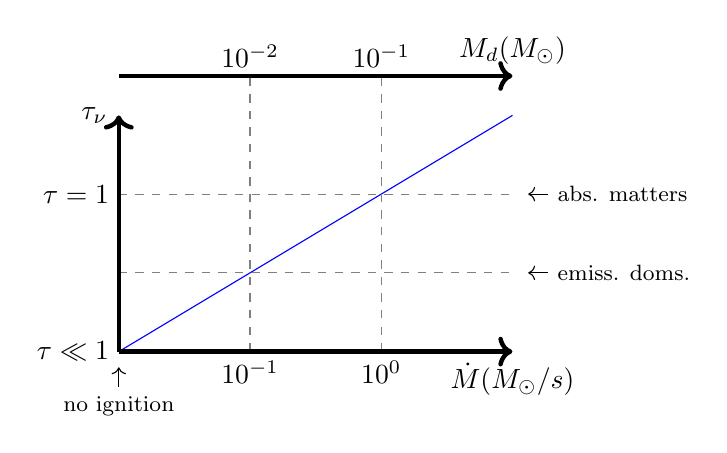
\begin{tikzpicture}
      \coordinate (origin) at (0,0);

      \draw[blue] (origin) -- (5,3);

      \node[left] (tau1) at (0,2) {$\tau=1$};
      \draw[dashed,gray] (tau1) -- ++(5.5,0);

      \node[below] (m1) at (10./3.,0) {$10^0$};
      \draw[dashed,gray] (m1) -- ++(0,3.75)
      node[above] {\color{black}$10^{-1}$};
      
      \coordinate(tau2) at (0,1);
      \draw[dashed,gray] (tau2) -- ++(5,0);

      \node[below](m2) at (5./3.,0) {$10^{-1}$};
      \draw[dashed, gray] (m2) -- ++(0, 3.75)
      node[above] {\color{black}$10^{-2}$};

      \node[left] at (origin) {$\tau\ll 1$};
      \draw[ultra thick, black,->] (origin)
      -- ++(5, 0) node[below] {$\dot{M} (M_\odot/s)$};
      \draw[ultra thick, black, ->] (origin)
      -- ++(0, 3) node[left] {$\tau_\nu$};
      \draw[ultra thick, black, ->] (0,3.5)
      -- ++(5,0) node[above] {$M_d (M_\odot)$};

      \draw[<-] (5.2,2) -- ++(0.25,0) node[right,align=left]
      {\footnotesize abs. matters};

      \draw[<-] (5.2,1) -- ++(0.25,0) node[right,align=left]
      {\footnotesize emiss. doms.};

      \draw[<-] (0,-0.2) -- ++(0,-0.25) node[below,align=center]
      {\footnotesize no ignition};
    \end{tikzpicture}
    }
\end{frame}

\begin{frame}
  \frametitle{Growth of Computing Power}
  \begin{center}
    \includegraphics[height=7cm,clip,trim={0 0 150 100}]{top500}
  \end{center}
  Top500 List
\end{frame}

\begin{frame}
  \frametitle{Parthenon: Unlocking GPU Cycles}
  \begin{columns}
    \begin{column}{6cm}
      \begin{center}
        \includegraphics[width=\columnwidth,clip,trim={0 0 150 100}]{top500}
      \end{center}
      {\footnotesize Top500 List}
    \end{column}
    \begin{column}{6cm}
      \begin{center}
        \includegraphics[height=6cm]{parth-hydro-scaling_weak}
      \end{center}
      {\footnotesize Grete, \textbf{JMM}, et al., ArXiv:2202.12309}
    \end{column}
  \end{columns}
\end{frame}

\begin{frame}
  \frametitle{Tools built on top of Parthenon}
  \begin{columns}
    \begin{column}{6cm}
      \begin{itemize}
      \item Phoebus, neutron star
      \end{itemize}
      \begin{center}
        \includegraphics[height=6cm]{tov_fig_paper}
      \end{center}
    \end{column}
    \begin{column}{6cm}
      \begin{itemize}
      \item Athena-PK, turbulence
      \end{itemize}
      \begin{center}
        \includegraphics[width=\columnwidth]{athenapk_sample}
      \end{center}
        \begin{itemize}
        \item Riot, triple point
        \end{itemize}
        \begin{center}
          \includegraphics[height=3cm]{triple}
        \end{center}
    \end{column}
  \end{columns}
  {\footnotesize Grete, \textbf{JMM}, et al., 2022}
\end{frame}

\begin{frame}
  \frametitle{Project Plan}
  \begin{itemize}
  \item \textbf{Plan:} Use new computing power unlocked by GPUs, and leverage the
    Phoebus/Parthenon codes built for the ASC program to model
    collapsars, fill in gaps in modeling.
  \item \textbf{Mission Relevance:} Lessons from Phoebus/Parthenon
    development can be applied to the weapons program.
    \begin{itemize}
    \item Fit neatly into ``Quarks-to-Cosmos'' focus of NPAC section
      of NPF pillar (note LDRD priorities have now changed)
    \item AMR, GPU, performance-portability. (See, e.g., talk at Salishan)
    \item Nuclear physics and reactions.
    \item Microphysics can be translated into XCAP project.
    \item Recruiting Pipeline.
    \end{itemize}
  \item \textbf{Risk:} ASC drops Phoebus, and it isn't ready
  \item \textbf{Mitigation:} Can use $\nu\texttt{bhlight}$ to attack
    r-process disk questions while we get Phoebus ready.
  \end{itemize}
\end{frame}

\begin{frame}
  \frametitle{Project: BH-NS Merger Disks}
  \begin{columns}
    \begin{column}{6cm}
      \begin{center}
        \includegraphics[height=3.5cm]{bhns_curtis/nsbh_disks_rho_ye_0}\\
        \includegraphics[height=3.5cm]{bhns_curtis/nsbh_disks_rho_ye_3}
      \end{center}
    \end{column}
    \begin{column}{6cm}
      \begin{itemize}
      \item BH-NS mergers can produce very massive, exotic disks
      \end{itemize}
      \begin{center}
        \includegraphics[width=6cm]{bhns_curtis/total_abun_disks_dec22}
        {\footnotesize Curtis, \textbf{JMM}, et al., ApJL 945 L13 (2023)}
      \end{center}
    \end{column}
  \end{columns}
\end{frame}

\begin{frame}
  \frametitle{Project: Varying Black Hole Parameters}
  \begin{columns}
    \begin{column}{4cm}
      \begin{center}
        \includegraphics[height=7cm]{valeria/3dsimplot_beta}
      \end{center}
    \end{column}
    \begin{column}{8cm}
      \begin{itemize}
      \item Investigate how jet opening angle varies with black hole spin
      \item Perhaps connects to long GRB properties for collapsars
      \end{itemize}
      \begin{center}
        \includegraphics[width=0.7\columnwidth]{valeria/thwsigbigger}
      \end{center}
      {\footnotesize Urrutia-Hurtado, Lloyd-Ronning, \textbf{JMM}, submitted to ApJL.}
    \end{column}
  \end{columns}
\end{frame}

\begin{frame}
  \frametitle{Project: Impact of Magnetic Field}
  \begin{itemize}
  \item Magnetically-driven turbulence drives angular momentum transport.
  \end{itemize}
  \begin{columns}
    \begin{column}{2.5cm}
      \begin{center}
        \includegraphics[height=6cm]{kelsey/4ms_comp}
      \end{center}
    \end{column}
    \begin{column}{9.5cm}
      \begin{itemize}
      \item Field must ``spin up'' due to turbulent instability.
      \item Larger fields mean less spin-up time, also more ``memory''
        of initial configuration.
      \item Impacts yields, outflow morphology.
      \end{itemize}
      \begin{center}
        \includegraphics[height=3cm]{kelsey/masses_wpercent}
      \end{center}
      {\footnotesize Lund, \textbf{JMM}, et al., submitted to ApJ.}
    \end{column}
  \end{columns}
\end{frame}

\begin{frame}
  \frametitle{Project: Ultra Late-Time Outflow}
  \begin{itemize}
  \item Original models of post-merger disks (and collapsars) only run
    for very short time: $\sim 120$ms.
  \item Outflow not finished by this time. Late-time outflow may look
    very different.
  \item Extended simulation to 1.2s physical time. 7 months required
    on supercomputer.
  \end{itemize}
  \begin{columns}
    \begin{column}{6cm}
      \begin{center}
        \includegraphics[width=0.9\columnwidth]{longsim/outflow_components}
      \end{center}
    \end{column}
    \begin{column}{6cm}
      \begin{center}
        \includegraphics[width=0.9\columnwidth]{longsim/ya_short_v_long}
      \end{center}
    \end{column}
  \end{columns}
  {\footnotesize Sprouse, \textbf{JMM}, et al., submitted to ApJ}
\end{frame}

\begin{frame}
  \frametitle{Project: Nuclear Uncertainties}
  \begin{itemize}
  \item Many uncertainties in nuclear reactions far from stability
  \item Do they ``wash out'' when averaged over an outflow with a continuum of conditions?
    \begin{itemize}
    \item No!
    \end{itemize}
  \end{itemize}
  \begin{columns}
    \begin{column}{6cm}
      \begin{center}
        \includegraphics[width=0.9\columnwidth]{nuclear-uncertainties/za_nuclear_geomean}
      \end{center}
    \end{column}
    \begin{column}{6cm}
      \begin{center}
        \includegraphics[width=0.9\columnwidth]{nuclear-uncertainties/corr_mass_ab}
      \end{center}
    \end{column}
  \end{columns}
  {\footnotesize Mumpower, Sprouse, \textbf{JMM}, in prep.}
\end{frame}

\begin{frame}
  \frametitle{Project: Neutrino Detectability}
  \begin{columns}
    \begin{column}{6cm}
      \begin{itemize}
      \item Neutrino luminosities from collapsars/NS Mergers likely too
        low to see with realistic rates and redshifts
      \item Nevertheless, interesting to ask what such an observation
        would look like if we were lucky enough to have an event occur in
        our local universe
      \item Primary collaborators: Matt Mumpower (T-2), Wendell Misch (XTD-PRI)
      \end{itemize}
    \end{column}
    \begin{column}{6cm}
      \begin{center}
        \includegraphics[width=0.9\columnwidth]{nuspec/nuspec_compare}
      \end{center}
    \end{column}
  \end{columns}
\end{frame}

\begin{frame}
  \frametitle{Spin-Off Project: Gravitational Waves from CCSN}
  \begin{itemize}
  \item Core collapse produces gravitational waves.
  \item Typically full 3D numerical relativity required, to capture.
  \item Now can extract eigenfrequencies though not intensities from
    spherically symmetric simulations
  \end{itemize}
  \begin{center}
    \includegraphics[height=5cm]{ccsn-eigenmodes/fmode-mpns-lines}
  \end{center}
  {\footnotesize Wolfe, \textbf{JMM}, et al., ApJ \textbf{954} 161 (2023)}
\end{frame}

\begin{frame}
  \frametitle{Spin-Off Project: $\nu$ Osscillations and Annihilation}
  \begin{itemize}
  \item Neutrinos can \textit{oscillate} from one flavor to
    another. This can impact nucleosynthesis.
  \item Due to length/time scales, impossible to treat from first principles
  \item Leverage $\nu\texttt{bhlight}$'s unprecedented accuracy in neutrinos to look for type of oscillation instability, fast flavor (Payel Mukhopadhyay)
  \item Similar techniques can be used to investigate contributions of
    $\nu-\bar{\nu}$ reactions to jet power (Sudipta Hensh).
  \end{itemize}
  \begin{columns}
    \begin{column}{6cm}
      \begin{center}
        \includegraphics[width=0.9\columnwidth]{payel/60-70km_fast_flavor_equator_radial}
      \end{center}
    \end{column}
    \begin{column}{6cm}
      \begin{center}
        \includegraphics[width=0.9\columnwidth]{payel/crossing_space}
      \end{center}
    \end{column}
  \end{columns}
\end{frame}

\begin{frame}
  \frametitle{Spin-Off Project: Supernovae in Phoebus}
  \begin{itemize}
  \item Graduate Student: Mariam Gogilashvili
  \item Connecting pen-and-paper model (FEC) to simulations: Gogilashvili, \textbf{JMM}, and Murphy, submitted to ApJ.
  \end{itemize}
  \begin{columns}
    \begin{column}{6cm}
      \begin{center}
        % \includegraphics[width=0.9\textwidth]{mgog_1d/frame_500}
        \animategraphics[width=0.9\textwidth,every=20,autoplay,loop,controls=off]
        {20}{mgog_1d/frame_}{001}{900}
      \end{center}
    \end{column}
    \begin{column}{6cm}
      \begin{center}
        \includegraphics[width=\columnwidth]{FECvsTime}
      \end{center}
    \end{column}
  \end{columns}
\end{frame}


\begin{frame}
  \frametitle{Next Steps: Phoebus is Ready!}
  \begin{itemize}
  \item Led by student, Brandon Barker at MSU
  \end{itemize}
  \begin{columns}
    \begin{column}{6cm}
      \begin{center}
        \includegraphics[width=0.9\textwidth]{tchekovskoy_initial_data/rho}
      \end{center}
      \begin{itemize}
      \item Initial density constructed as parametrized model of collapse
      \end{itemize}
    \end{column}
    \begin{column}{6cm}
      \begin{center}
        % \includegraphics[width=0.9\textwidth]{phoebus_movies/tracers_torus/frame_0761}
        \animategraphics[width=0.9\textwidth,every=10,autoplay,loop,controls=off]
        {10}{phoebus_movies/tracers_torus/frame_}{0001}{0761}
      \end{center}
      \begin{itemize}
      \item Compact torus with Monte Carlo rad, MHD, and tracer particles
      \end{itemize}
    \end{column}
  \end{columns}
\end{frame}

\begin{frame}
  \frametitle{Publications And Status}
  \begin{itemize}
  \item Published
    \begin{itemize}
    \item Curits et al., ApJL \textbf{945} (1), L13 (2023)
    \item Wolfe et al., ApJ \textbf{954} (2), 161 (2023)
    \item Barker et al., ApJL \textbf{944}, L2 (2023)
    \item Turk et al., Manubrot, (2023)
    \end{itemize}
  \item Reviewed favorably, published soon
    \begin{itemize}
    \item Gogilashvili et al, \textit{To ApJ}
    \item Urrutia-Hurtado et al., \textit{To ApJL}
    \item Sprouse et al., \textit{To ApJ}
    \item Fryer et al., \textit{To ApJ}
    \item Lund et al., \textit{To ApJ}
    \end{itemize}
  \end{itemize}
\end{frame}

\begin{frame}
  \frametitle{Projects In-Flight/In-Prep}
  \begin{itemize}
  \item In Prep.
    \begin{itemize}
    \item Barker et al., \textit{To ApJS}
    \item Mumpower et al., \textit{To ApJ}
    \end{itemize}
  \item Projects in-flight:
    \begin{itemize}
    \item Barker---First full collapsar simulation with Phoebus
    \item Lund---Impact of magnetic field topology
    \item Mukhopadhyay---Neutrino oscillations
    \item Hensh---Neutrino annihilation
    \item Mumpower + Misch---Observability of NS merger and
      collapsar events in next-gen neutrino detectors
    \end{itemize}
  \item Follow-On Funding
    \begin{itemize}
    \item Gogilashvili---CCSNe simulations
    \item Fields + Murphy---NSF cyberinfrastructure grant for Phoebus
    \item Lund---Multi-messenger inference for nuclear EOS
    \end{itemize}
  \end{itemize}
\end{frame}

\begin{frame}
  \frametitle{Workforce Development in Project}
  \begin{itemize}
  \item PI Developed own and lab reputation through publications,
    collaborations, talks and conferences
  \item PI Managed own time as well as student time accross variety of
    sub-projects
  \item PI time spent mentoring:
    \begin{itemize}
    \item 1 Student fully funded by project
    \item 2 Students not funded by project
    \end{itemize}
  \item PI collaborated/maintained relationships with:
    \begin{itemize}
    \item 2 Former LANL students, one now a postdoc at Berkely, one
      now a graduate student at University of Washington
    \item 1 Former LANL postdoc, now in industry
    \item 2 non-LANL postdocs, who may be interested in the laboratory
    \item 1 Graduate student at MIT
    \end{itemize}
  \end{itemize}
\end{frame}

\begin{frame}
  \frametitle{Conclusions}
  \begin{columns}
    \begin{column}{7cm}
      \begin{itemize}
      \item The heaviest elements in the universe produced in NS mergers and maybe collapsars
        \begin{itemize}
        \item Need GRRMHD and neutrino transport!
        \item Systems remarkably similar
        \end{itemize}
      \item Risk in proposal came to pass--Phoebus was not ready
      \item Risk effectively mitigated, and project remarkably productive:
        \begin{itemize}
        \item Many high-impact publications and talks
        \item Trained students
        \item Experience can translate back to the program
        \end{itemize}
      \end{itemize}
    \end{column}
    \begin{column}{5cm}
      \includegraphics[width=\columnwidth,clip,trim={150 0 150 0}]{3d_render}
    \end{column}
  \end{columns}
\end{frame}

\backupbegin

\backupend

\end{document}